\documentclass{article}


% if you need to pass options to natbib, use, e.g.:
%     \PassOptionsToPackage{numbers, compress}{natbib}
% before loading neurips_2023


% ready for submission
\usepackage[final]{neurips_2023}


% to compile a preprint version, e.g., for submission to arXiv, add add the
% [preprint] option:
%     \usepackage[preprint]{neurips_2023}


% to compile a camera-ready version, add the [final] option, e.g.:
%     \usepackage[final]{neurips_2023}


% to avoid loading the natbib package, add option nonatbib:
%    \usepackage[nonatbib]{neurips_2023}


\usepackage[utf8]{inputenc} % allow utf-8 input
\usepackage[T1]{fontenc}    % use 8-bit T1 fonts
\usepackage{hyperref}       % hyperlinks
\usepackage{url}            % simple URL typesetting
\usepackage{booktabs}       % professional-quality tables
\usepackage{amsfonts}       % blackboard math symbols
\usepackage{nicefrac}       % compact symbols for 1/2, etc.
\usepackage{microtype}      % microtypography
\usepackage{xcolor}         % colors
\usepackage{graphicx}       % images
\usepackage{float}          % use the [H] option for figure placement


\title{Project Proposal: Transformer-based Model for Mathematical Problem Solving}


% The \author macro works with any number of authors. There are two commands
% used to separate the names and addresses of multiple authors: \And and \AND.
%
% Using \And between authors leaves it to LaTeX to determine where to break the
% lines. Using \AND forces a line break at that point. So, if LaTeX puts 3 of 4
% authors names on the first line, and the last on the second line, try using
% \AND instead of \And before the third author name.


\author{%
    Chau Nguyen \\
    \texttt{chauminh.nguyen@mail.utoronto.ca} \\
    \and
    Gabriel You \\
    \texttt{gabriel.you@mail.utoronto.ca} \\
    \and
    Takia Talha \\
    \texttt{takia.talha@mail.utoronto.ca} \\
    \and
    Taha Siddiqi \\
    \texttt{taha.siddiqi@mail.utoronto.ca} \\
    \\
    Department of Mathematical \& Computational Sciences \\
    University of Toronto Mississauga
}
\begin{document}

\maketitle


\begin{abstract}
%   Chloe

%   The abstract paragraph should be indented \nicefrac{1}{2}~inch (3~picas) on
%   both the left- and right-hand margins. Use 10~point type, with a vertical
%   spacing (leading) of 11~points.  The word \textbf{Abstract} must be centered,
%   bold, and in point size 12. Two line spaces precede the abstract. The abstract
%   must be limited to one paragraph.

%   A short description of your goals, task, model, and (for
% the final report) results. The abstract should make the
% motivations and the scope of your project clear so that
% readers can decide whether they are interested in
% reading your work.
  Mathematical problem solving often requires both symbolic manipulation and natural language understanding. In this paper, we propose a hybrid, lightweight, and open-source model that combines symbolic mathematics with deep learning to solve mathematical problems expressed in natural language or LaTeX format. Our approach integrates several powerful components: \texttt{LaTeX2SymPy} for parsing mathematical expressions from LaTeX, \texttt{MathBERT} for tokenizing and encoding both natural language and symbolic math content, \texttt{SymPy} for symbolic computation and exact mathematical solving, and a Seq2Seq decoder for generating natural language output from symbolic results. This architecture allows the model to handle complex mathematical reasoning tasks, from simple algebraic equations to advanced calculus, while providing accurate and interpretable solutions. The model is efficient, scalable, and entirely open-source, enabling easy integration into educational tools, computational software, and research applications. We demonstrate that our hybrid model leverages the strengths of both symbolic and neural approaches to deliver a more robust solution for automated math problem-solving.
  \end{abstract}
\section{Introduction}
% Gabriel

% A description of the motivation behind your work, why
% the task you chose is interesting/important, and a
% summary of your (proposed) approach. The problem
% that you want to solve should be clearly stated in the
% introduction: especially the input and output of your
% model and the format of the input and output. This
% section should also make it clear why your deep
% learning approach is reasonable for this problem.
A challenge often faced by students in the computational sciences 
is learning how to solve logically intensive math questions. 
Often times the transition from computation focused math to reasoning 
focused math presents a large learning curve due to the difficulty of 
developing mathematical intuition and a lack of rigorous step by step 
answers to compare with. We hope to develop an accessible model that can 
take in a latex text input of a math problem and output a descriptive and accurate latex text answer output to the problem. 
Developing models capable of solving this task is an infamously difficult problem \cite{Ünsal_Gehr_Vechev_2024} due to the requirement of consistency and mathematical riqour within the answers outputted by the models. 
\\
Currently the best models in this area use transformer LLM archetictures with large pretraining datasets. 
The downsides of these models is that the consistency may be poor due to multiple ways to present the same problem which are treated differently by the model.
To solve for this we are incorporating a symbolic model into a transformer LLM architecture to hopefully increase accuracy within our math solving model.
 We believe this deep learning approach is reasonable as understanding the language of math problems is something suited for transformer LLM models and creating consistency in mathematical reasoning is something that symbolic models are good at. By combining these 2 approaches we hope that it will combine the best of both architectures.  With this work we hope to develop a more robust and helpful model that is able to answer with reason and provide thorough feedback on math questions potential users might have.

 \section{Background and Related Work}
% Chloe

% A summary of the background material that students of
% CSC413 would not already be familiar with. A
% description of related work done in the area, and how
% your approach compares with theirs.

% If your project builds on previous work, clearly
% distinguish what they did from what your new
% contribution is. Also, include a 1-2 sentence summary
% of other closely related papers. We realize you might
% not know about all related papers (or have time to
% carefully read all related papers), and that's OK for this
% project. Using bibtex is annoying at first, but Google
% Scholar can give you the bibtex entries.

The application of large language models (LLMs) such as BERT \cite{mathBERT} and GPT \cite{Brown_et_al._2020} has revolutionized the field of natural language processing (NLP). These transformer-based models excel at a wide range of tasks, including text classification, question answering, and translation. However, when it comes to mathematical reasoning and algebraic problem solving, LLMs often face challenges due to their primary design focusing on natural language rather than symbolic or mathematical computation.

To address this, there has been increasing interest in integrating symbolic reasoning capabilities into neural architectures. Symbolic models are traditionally used for tasks that require formal manipulation of symbols, such as equation solving, logical inference, and symbolic differentiation. Recent efforts have focused on combining the power of neural networks with symbolic reasoning systems to enhance the models' performance on tasks that involve mathematics or formal logic.

\subsection{The Role of Symbolic Models in Mathematical Reasoning}

Symbolic models have long been a central tool in areas such as algebra, calculus, and theorem proving. These models represent mathematical objects (e.g., variables, equations, operators) explicitly and can apply algebraic rules, differentiation, integration, and other symbolic operations directly to manipulate these objects. However, traditional symbolic approaches face scalability issues when dealing with large, unstructured datasets, such as those encountered in real-world mathematical problem solving. 

On the other hand, neural networks, particularly deep learning models, excel at processing unstructured data like natural language and images. Yet, they often struggle with the step-by-step logical reasoning required for tasks like algebraic equation solving or symbolic manipulation due to their inability to explicitly model mathematical operations. This limitation has motivated research into hybrid approaches that combine the benefits of both symbolic models and neural architectures.

\subsection{Integration of Symbolic Models into Transformer-based Architecture}

Recent work has explored the integration of symbolic reasoning within Large Language Models, particularly in the context of mathematical problem solving. A key idea is to augment traditional neural models with external symbolic components that can handle explicit algebraic operations. For example, incorporating \textit{symbolic equation solvers} into a Generative Pretrained Transformer (GPT) allows neural networks to handle more complex algebraic problems \cite{Hu2022Enhancing}. However, GPTs and other Large Language Models are large and not open-source, which makes it challenging for nonprofit educational organizations to conduct research and deploy it effectively due to limited access, high computational costs, and restrictions on customization.

On the other hand, Bidirectional Encoder Representations from Transformers (BERT), originally designed for NLP tasks, has been shown to benefit from fine-tuning on an extensive and diverse mathematical corpuses. Devlin et al. (2024) proposed the finetuning of BERT on mathematical datasets to better understand and solve algebraic problems \cite{DevlinBERT}. Given that BERT and its variants, including mathBERT, are open source, lightweight and accessible to the general public, research and development in extending its current performance would be more easily motivated and conducted. However, to handle more complex mathematical reasoning tasks that involve symbolic manipulation, BERT-based models can be augmented with symbolic reasoning modules that perform operations like solving equations, simplifying expressions, and computing symbolic derivatives. This approach attempts to overcome the limitations of pure neural models by integrating symbolic computations into the reasoning process of the model. 

Recent advances have focused on combining symbolic models with large language models to improve their ability to solve algebraic problems. In the context of BERT and similar models, symbolic models can be incorporated into the encoder-decoder structure, either by pre-processing mathematical inputs with symbolic solvers or by augmenting the model's latent space with symbolic representations that guide its reasoning. For example, the work by Ünsal et al. \cite{Ünsal_Gehr_Vechev_2024} introduces a method where symbolic expressions produced by symbolic models are integrated directly into the attention mechanism of transformer-based models, allowing the network to learn from an accurate chain of subexpressions as part of the mathematical solving procedure as if they were a a paragraph composed of sentences.

\subsection{Contributions of the Current Work}

In this work, we propose a novel approach to algebraic problem solving by incorporating a symbolic model into the BERT encoder. We aim to enhance the BERT architecture with an external symbolic solver that can manipulate algebraic expressions, perform equation solving, and reason about mathematical objects symbolically. By integrating these symbolic capabilities directly into the BERT encoder, we hypothesize that the model will achieve improved performance on algebraic problem-solving tasks, enabling it to generate both correct and interpretable solutions to complex algebraic problems. Our work builds on recent advances in symbolic-augmented language models and aims to push the boundaries of what is achievable in algebraic reasoning within LLMs.


\section{Data}
% Taha 

% The dataset used in your model. Include any key
% exploratory figures that will help readers evaluate the
% difficulty of your problem and interpret the performance
% of your model.

\subsection{Datasets}

For this project, we decided to use the following datasets:

\href{https://www.kaggle.com/datasets/mathurinache/math-dataset}{{\bf Math Dataset}}

The MATH dataset consists of 12,500 (7,500 training and 5,000 test) problems from mathematics competitions including the AMC 10, AMC 12, AIME, and more. Many of these problems can be collected from \href{https://artofproblemsolving.com/community/c3158\_usa\_contests}{aops.com/community/c3158\_usa\_contests}.
\cite{hendrycksmath2021}

\href{https://huggingface.co/datasets/AI-MO/NuminaMath-CoT}{{\bf NuminaMath-CoT}}

The Numina Math CoT dataset has approximately 860k math problems, where each solution is formatted in a Chain of Thought (CoT) manner. The sources of the dataset range from Chinese high school math exercises to US and international mathematics olympiad competition problems.
\cite{numina_math_datasets_CoT}

\href{https://huggingface.co/datasets/AI-MO/NuminaMath-TIR}{{\bf NuminaMath-TIR}}

The Numina Math TIR dataset is a more specific version of the CoT dataset, where 70k problems are selected, with a focus on numerical outputs and integers. Tool-integrated reasoning (TIR) plays a crucial role in this dataset, where the solution to each problem is a sequence of steps that can be executed by a computer program.
\cite{numina_math_datasets_TIR}

\subsection{Data Formatting}

Problems and solutions are formatted using LATEX. The usage of LATEX ensures that the data is easily readable and is easy to parse and process for training the model.

The data for the Math Dataset is formatted as a JSON file, with each problem containing the following fields:
\begin{itemize}
  \item problem: The text of the problem
  \item level: The difficulty level of the problem (Level 1 up to Level 5)
  \item type: The type of math problem (e.g. algebra, geometry, etc.)
  \item solution: The solution to the problem
\end{itemize}

The data for the Numina Math CoT and TIR datasets are formatted as a JSON file, with each problem containing the following fields:
\begin{itemize}
  \item An array of objects, where the first object contains
      \begin{itemize}
        \item content: The text of the problem
        \item role: the role assigned to the person who can access this data (user)
      \end{itemize}
  \item The second object contains
      \begin{itemize}
        \item content: The solution to the problem
        \item role: the role assigned to the person who can access this data (assistant)
      \end{itemize}
\end{itemize}

We intend to use these datasets to train our model to solve mathematical problems. We will preprocess the data into one format, to ensure that can be used by our model. We will also split the test data into validation and test sets to evaluate the performance of our model.

\section{Model Architecture}

The proposed model aims to combine the strengths of symbolic math-solving with neural language understanding by utilizing a hybrid architecture that integrates \texttt{LaTeX2SymPy} for parsing mathematical expressions, the \texttt{mathBERT} tokenizer and encoder for understanding the natural language problem, \texttt{SymPy} for symbolic manipulation and computation, and a Seq2Seq decoder for generating textual output. The architecture is designed to be lightweight, efficient, and open-source, making it accessible for deployment in a wide range of applications.

\subsection{Input Layer: LaTeX2SymPy Parsing}

The input to the model is a natural language mathematical problem, often expressed in LaTeX format. To handle the structured mathematical expressions present in LaTeX format, we use \texttt{LaTeX2SymPy}. This component parses the LaTeX input into a symbolic expression that can be processed by the subsequent layers.

\begin{itemize}
    \item \textbf{LaTeX Parsing:} Convert LaTeX-based input strings into tokenized symbolic expressions.
    \item \textbf{Symbolic Representation:} Map the parsed LaTeX expressions into \texttt{SymPy} objects, which represent mathematical terms, operators, and functions in a format suitable for algebraic manipulation.
\end{itemize}

This parsing step ensures that the mathematical problem is represented in a structured and mathematically accurate form, making it ready for further symbolic operations.

\subsection{SymPy Solver}

Once the problem is tokenized and embedded by the MathBERT encoder, it is passed to the \texttt{SymPy} Solver for symbolic computation. \texttt{SymPy} is a Python library dedicated to symbolic mathematics, and its role in this architecture is twofold:

\begin{itemize}
    \item \textbf{Symbolic Manipulation:} \texttt{SymPy} is used to perform algebraic simplifications, differentiation, integration, solving equations, and other symbolic manipulations based on the parsed mathematical expression. This step leverages the full symbolic capabilities of \texttt{SymPy} to compute exact solutions when possible.
    \item \textbf{Mathematical Inference:} For problems requiring a numerical solution (such as solving equations), \texttt{SymPy} can use numerical solvers to provide an approximate answer. \texttt{SymPy} supports a wide range of operations, ensuring that the model can handle complex algebraic, calculus, and number-theoretic problems.
    \item \textbf{Generation of Subexpressions} The SymPy solver processes a given function one step at a time. To simulate the process of arriving at a mathematical solution, we feed the given expression into SymPy, then repeatedly feed the output expression into the SymPy until a solution is arrived. The generated subexpressions are sequentially concatenated in the order that they are produced, and the final string is passed into the tokenizer. The goal is for the model to not only learn the positional embeddings and the underlying relations behind the word and mathematical expression parts of a given problem, but also to learn the explicit steps leading up to the solution. 
\end{itemize}

This integration ensures that the model not only understands the mathematical structure of the problem but also can derive precise and reliable solutions when applicable.

\subsection{MathBERT Tokenizer and Encoder}

The parsed mathematical expression is fed into a \texttt{MathBERT} tokenizer and encoder, which is a specialized version of BERT fine-tuned for mathematical tasks \cite{mathbert}. MathBERT has been trained to handle both natural language and symbolic mathematical notation, which allows it to effectively process math-related queries and understand the underlying structure of the problem. The steps involved are as follows:

\begin{itemize}
    \item \textbf{Tokenization:} The \texttt{MathBERT} tokenizer splits the input into subword tokens that represent both natural language components and mathematical symbols. This step is crucial for handling mixed inputs such as text-based questions and mathematical formulas.
    \item \textbf{Contextual Embedding:} The tokenized input is passed through the \texttt{MathBERT} encoder, which generates contextual embeddings for each token. These embeddings capture semantic relationships between mathematical operations, variables, and their corresponding natural language descriptions. The encoder's attention mechanism enables the model to focus on relevant parts of the input when generating solutions.
\end{itemize}

\subsection{Seq2Seq Decoder}

The final step of the architecture involves the use of a Seq2Seq decoder, which generates the natural language output from the symbolic solution obtained from \texttt{SymPy}. The decoder is designed to convert symbolic results back into human-readable text, making the solution interpretable and usable for end-users.

\begin{itemize}
    \item \textbf{Input:} The output from \texttt{SymPy} (whether symbolic or numeric) is used as input to the decoder.
    \item \textbf{Generation:} The Seq2Seq model is trained to map the symbolic solution into a sequence of natural language words or sentences. This component ensures that the model can output the solution in an understandable and grammatically correct format.
\end{itemize}

This step integrates both symbolic manipulation and natural language generation, ensuring that the solution is not only mathematically accurate but also linguistically appropriate.

\subsection{Advantages of the Proposed Architecture}

The hybrid architecture offers several advantages:

\begin{itemize}
    \item \textbf{Hybrid Approach:} The combination of symbolic computation (via \texttt{SymPy}) and deep learning (via \texttt{MathBERT} and Seq2Seq) leverages the strengths of both methods, enabling the model to handle complex mathematical reasoning and natural language understanding simultaneously.
    \item \textbf{Lightweight and Efficient:} The model is designed to be efficient by using pre-trained BERT embeddings and leveraging \texttt{SymPy} for exact symbolic computation, reducing the need for large-scale numerical solvers or extensive training data.
    \item \textbf{Open Source:} All components of the model (\texttt{SymPy}, \texttt{MathBERT}, Seq2Seq, and \texttt{LaTeX2SymPy}) are open-source, ensuring transparency, reproducibility, and accessibility.
    \item \textbf{Scalability:} The model can handle a wide variety of mathematical problems, from basic algebra to more advanced calculus and number theory, making it suitable for a range of educational and professional applications.
\end{itemize}


\section{Model architecture figure}
% Takia

% A figure that helps show the overall model or idea. The
% idea is to make your paper more accessible, especially
% to readers who are starting by skimming your paper.
% You must create a new figure, not just use someone
% else's, even with attribution. Be careful that all figure
% text are legible, and are approximately the same size
% as the main text.

\begin{figure}[H]
  \centering
  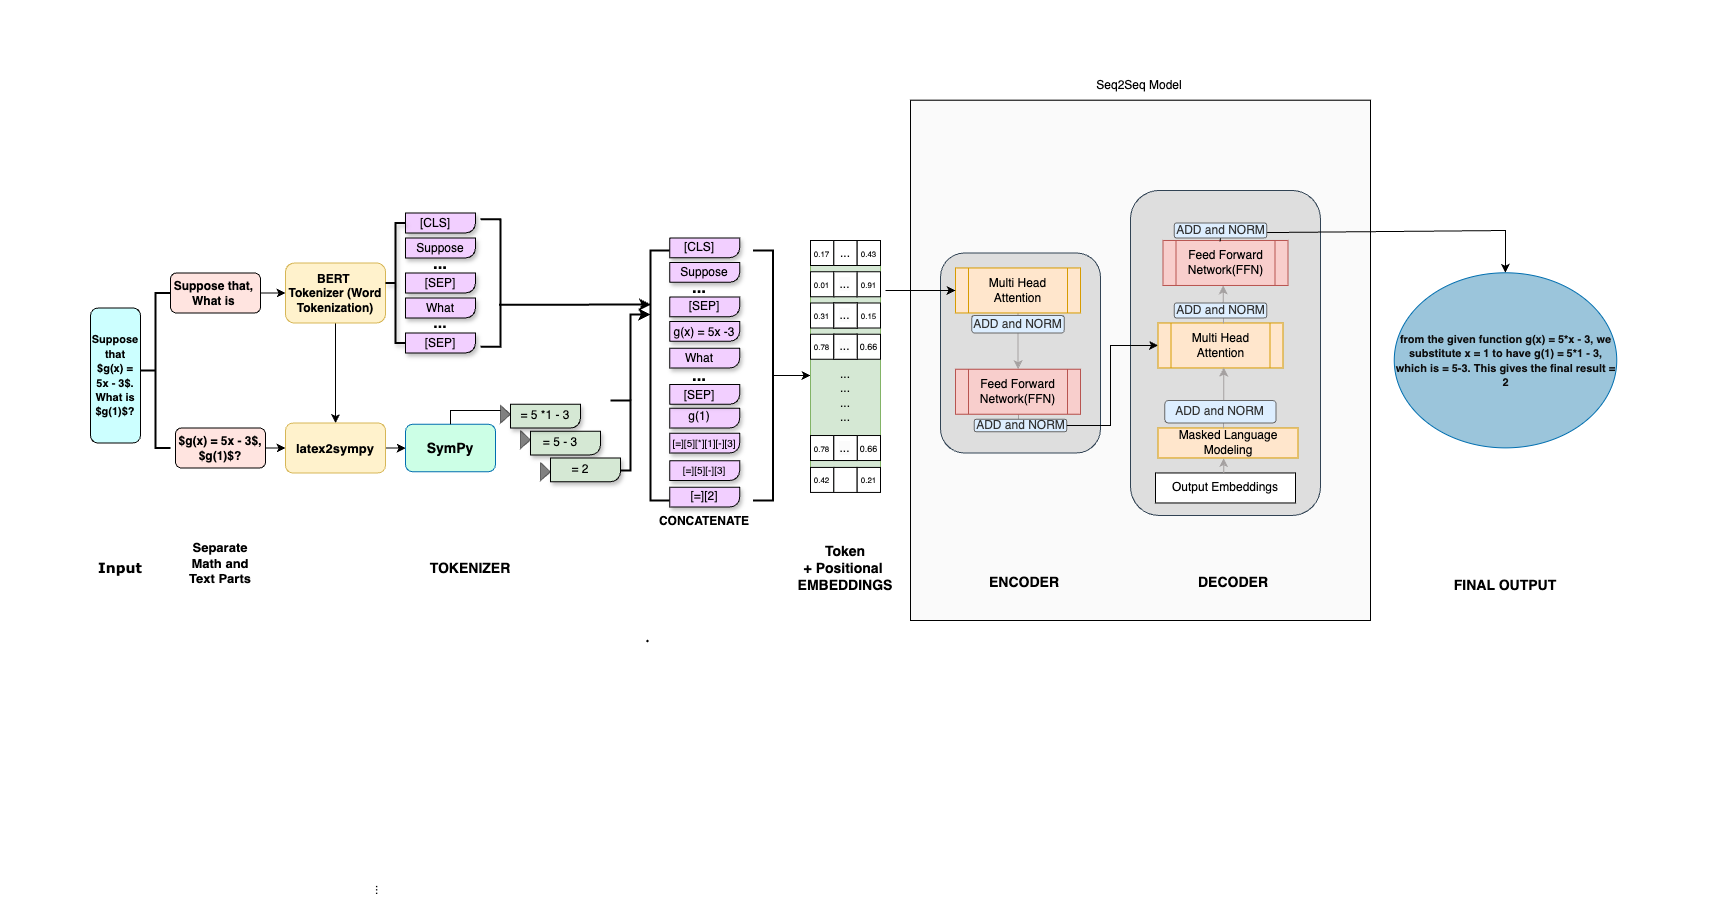
\includegraphics[scale=0.2]{./figures/Model_architecture_figure.png}
  \caption{The Transformer - model architecture.}
  \label{fig:model-arch}
\end{figure}


% LEAVE FOR FINAL REPORT
% \section{Results}
% Describe the performance of your model, either
% quantitatively or (for generative models) qualitatively. To
% help interpret the model, compare your model with a
% baseline model. Qualitative evaluation is OK.


% LEAVE FOR FINAL REPORT
% \section{Discussion}
% Interpret the results of your model. If appropriate,
% compare the model performance with the baseline.
% Discuss other features that you notice about the model.


% LEAVE FOR FINAL REPORT
% \section{Limitations}
% Describe some settings in which we’d expect your
% approach to perform poorly, or where all existing
% models fail. Try to guess or explain why these
% limitations are the way they are. Give some examples
% of possible extensions, ways to address these
% limitations or open problems

\section{Ethical considerations}
% Taha

% Potential ethical issues posed by the use or misuse of
% your model. Your report should transparently
% communicate the known or anticipated consequences
% of building and using machine learning models on this
% task.

% https://neurips.cc/public/EthicsGuidelines

\subsection{Ethical Issues}
One ethical consideration is the potential for the model to be used to cheat on math assignments/homework. This could encourage students to use the model as a shortcut rather than engaging with the material themselves, which would negatively impact a students capacity for critical thinking and problem-solving. 

Another ethical issue is intellectual property rights, as the model is trained on copyrighted data. The model could inadvertently promote plagiarism if it directly provides solutions that students submit as their own, without understanding the learning process. This could lead to academic dishonesty and undermine the integrity of the educational system.

\subsection{Mitigation Strategies}
To mitigate the first risk, the model should be used as a learning tool rather than a tool for cheating. For example, the model could be used to generate practice problems for students to solve, or to provide explanations for the solutions to problems. This would help students learn and improve their math skills, rather than using the model to cheat. Therefore, while automation can support learning, it is essential that it complements, rather than replaces, active engagement with the educational process.

To mitigate the second risk, the model should be used in a controlled environment where students are guided on how to use the model appropriately. For example, teachers could provide guidelines on how to use the model to check answers or generate practice problems, rather than using it to directly provide solutions. Furthermore, it is crucial to emphasize the value of understanding the material and using tools as aids rather than shortcuts. This would prevent plagiarism and encourage students to engage with the material and develop their problem-solving skills.

\section{Work division}
% #TODO: change work division to be that of the actual project
% A description of how the work will be divided between
% the team members, and how the team members will be
% working together (e.g. meet every week Tuesday 4-5
% pm).

\section*{Writing Components}
The work will be split as follows:
\begin{itemize}
  \item \textbf{Chloe} - Background and Related Work, Abstract, Model Architecture, Results
  \item \textbf{Takia} - Model Architecture Figure, Model Architecture, Discussions
  \item \textbf{Gabriel} - Introduction, Model Architecture, Conclusion
  \item \textbf{Taha} - Data, Ethical Considerations, Model Architecture, Limitatations
\end{itemize}

The team will work on each part and meet every weekend for additional discussions.

\section*{Technical Section}

\subsection*{Data-Related Tasks (Taha)}
\begin{itemize}
  \item Collecting and cleaning large datasets.
  \item Tokenizing text data.
  \item Creating and managing training, validation, and test datasets.
\end{itemize}

\subsection*{Model Architecture and Development Tasks (Chloe)}
\begin{itemize}
  \item Designing the encoder and decoder architecture.
  \item Implementing the transformer model (attention mechanisms, multi-head attention, etc.).
  \item Ensuring model components (BERT, etc.) work seamlessly together.
\end{itemize}

\subsection*{Training and Optimization (Gabriel)}
\textbf{Responsibilities:}
\begin{itemize}
  \item Setting up the training pipeline.
  \item Hyperparameter tuning (learning rate, batch size, etc.).
  \item Implementing and testing various optimization techniques (Adam, gradient clipping, learning rate schedules).
\end{itemize}

\subsection*{Evaluation and Visualizations (Takia)}
\textbf{Responsibilities:}
\begin{itemize}
  \item Evaluating model performance using appropriate metrics (BLEU score, perplexity).
  \item Developing visualization tools to monitor training and validation performance.
  \item Deciding what metrics to measure the model on.
\end{itemize}



% LEAVE FOR FINAL REPORT
% \section{Conclusion}

% A description of how the work will be divided between
% the team members, and how the team members will be
% working together (e.g. meet every week Tuesday 4-5
% pm).

\bibliographystyle{unsrt}
\bibliography{references}

\end{document}